\section{Concurrent programming}
Concurrency is an essential concept in computer science that enables multiple tasks to run simultaneously in a program.
This section introduces the concept of concurrent programming and discusses the different concepts associated with it.


\subsection{Throughput and Latency}
In sequential programming measuring the performance of a program can be done through measuring its execution time.
This can be acheived by recording the time when the program starts and when it finishes, and calculating the difference.
The througput then becomes the

The impact of future optimizations can then be measured by comparing the execution times before and after the optimizations are applied.
As the number of tasks that can be solved in a given time is

However, in concurrent processing, execution times of individual instructions may overlap, making it challenging to calculate the execution time of the individual instructions \cite[21]{volkovLatencyHiding2016}.
The same type for time measurements can still be performed, but i

Instead, metrics such as latency, throughput, and concurrency can be used to characterize the process.

For example, latency is the average time between the start and end times of individual items, while throughput is the number of items processed within a given time interval divided by the duration of the interval.
Concurrency is the number of items processed simultaneously and can be measured at different moments in time or as an average over a particular interval.


\subsection{Sequential programming}
To understand concurrent programming, we must first understand sequential programming.
Sequential programming is a programming paradigm in which one task is finished before the next one is started.
This can be seen as the default type of programming where one line of code is executed after another in a linear order.
Figure \ref{fig:concurrency_sequential} shows an example of sequential program that executes a sequence of three tasks multiple times.

\begin{figure}[H]
    \centering
    
\includegraphics[width=\textwidth]{figures/concurrency/sequential.pdf}
    \caption{Sequential programming}
    \label{fig:concurrency_sequential}
\end{figure}

If there is no reason to execute tasks concurrently, then sequential programming is often the best choice as there is little to no overhead involved and it is easy to understand, debug and maintain.

\subsection{Concurrent programming}
Concurrent programming is a programming paradigm in which multiple tasks are executed simultaneously, instead of in a sequential manner.


Concurrent programming can be split into two categories, asynchronous and parallel.


\subsection{Asynchronous programming}
Asynchronous programming is a programming paradigm in which tasks are executed concurrently without blocking the execution of other tasks.
In an asynchronous program, tasks are typically executed in a non-blocking manner, allowing the program to continue executing while waiting for the results of a particular task.

Asynchronous programming is often used in systems that perform I/O operations, such as network communication or file I/O, where waiting for the results of an operation can be time-consuming.
Rather than blocking the program until the operation is complete, an asynchronous program can execute other tasks while waiting for the operation to complete.

Asynchronous programming can be achieved through various techniques, including callbacks, promises, and async/await syntax.
With callbacks, a function is called when an asynchronous operation is completed, while promises provide a more structured way of handling asynchronous operations by allowing for the chaining of multiple operations.
The async/await syntax provides a more concise way of writing asynchronous code by using keywords to indicate that a function is asynchronous and that it is awaiting the completion of a particular operation.

Asynchronous programming is becoming increasingly important in modern software development, as it can improve the performance and scalability of applications, particularly in systems that involve large amounts of I/O operations.
However, it can be challenging to write and debug asynchronous code, as developers must be careful to avoid race conditions and other synchronization issues.
\begin{figure}[H]
    \centering
    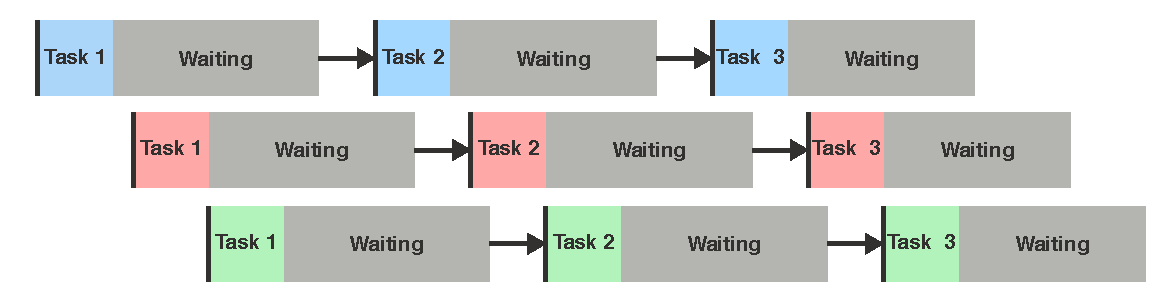
\includegraphics[width=\textwidth]{figures/concurrency/concurrent.pdf}
    \caption{Concurrent programming involving waiting}
    \label{fig:concurrency_concurrent}
\end{figure}

\subsection{Parallel programming}

Parallel programming is a programming paradigm in which multiple tasks or parts of a program are executed simultaneously on multiple processors or cores, with the goal of improving the performance and efficiency of the program.
In a parallel program, tasks can be divided into smaller sub-tasks that can be executed concurrently, potentially reducing the overall time required to complete the task.

Parallel programming can be achieved through various techniques, including multithreading, multiprocessing, and distributed computing.
Multithreading involves running multiple threads of execution within a single process, while multiprocessing involves running multiple processes in parallel.
Distributed computing involves running parts of a program on multiple machines connected through a network.

Parallel programming can provide significant performance benefits in systems that are designed to take advantage of multiple processors or cores.
However, designing parallel programs can be challenging, as developers must carefully manage resources and avoid synchronization issues, such as race conditions and deadlocks.

Parallel programming is becoming increasingly important in modern software development, as the number of cores and processors in computers and other devices continues to increase, and as more applications are designed to take advantage of parallel processing.
It is particularly important in areas such as scientific computing, data analysis, and artificial intelligence, where large amounts of data must be processed in a timely manner.

\pagebreak

\subsection{Parallelism}
Parallelism is a form of concurrency that involves executing multiple tasks simultaneously on different processors.


